\documentclass[10pt,a4paper]{article}

% ─── Packages ───────────────────────────────────────────────────────────────
\usepackage[margin=0.7in]{geometry}
\usepackage{graphicx}
\usepackage{titlesec}
\usepackage{fancyhdr}
\usepackage{setspace}
\usepackage{booktabs}
\usepackage{array}
\usepackage{listings}
\usepackage[table]{xcolor}
\usepackage{hyperref}
\usepackage{enumitem}
% \usepackage{parskip}
\usepackage{amsmath}
\usepackage{caption}
\usepackage{float}
\usepackage{newtxtext,newtxmath}
\usepackage{tikz}
\usetikzlibrary{arrows.meta,positioning}

% ─── Colours & Code Style ───────────────────────────────────────────────────
\definecolor{codebg}{RGB}{245,245,245}
\definecolor{codecomment}{RGB}{100,100,100}
\definecolor{codekeyword}{RGB}{0,0,200}
\definecolor{codestring}{RGB}{163,21,21}
\definecolor{accentblue}{RGB}{0,70,140}

\lstdefinestyle{arduino}{
  backgroundcolor=\color{codebg},
  commentstyle=\color{codecomment}\itshape,
  keywordstyle=\color{codekeyword}\bfseries,
  stringstyle=\color{codestring},
  basicstyle=\ttfamily\scriptsize,
  breakatwhitespace=false,
  breaklines=true,
  captionpos=b,
  keepspaces=true,
  numbers=none,
  numbersep=6pt,
  numberstyle=\tiny\color{gray},
  showspaces=false,
  showstringspaces=false,
  showtabs=false,
  tabsize=2,
  frame=single,
  framerule=0.5pt,
  rulecolor=\color{gray!50}
}

% ─── Section Formatting ─────────────────────────────────────────────────────
\titleformat{\section}{\normalsize\bfseries\color{accentblue}}{}{0em}{\thesection\quad}[\titlerule]
\titleformat{\subsection}{\small\bfseries}{}{0em}{\thesubsection\quad}
\titlespacing*{\section}{0pt}{8pt}{4pt}
\titlespacing*{\subsection}{0pt}{6pt}{3pt}
\setlength{\parskip}{2pt}
\setlength{\parindent}{0pt}
\setlist{nosep}

% ─── Header / Footer ────────────────────────────────────────────────────────
\pagestyle{fancy}
\fancyhf{}
\rhead{\small IoT-Based Smart Helmet}
\lhead{\small Lab Report}
\cfoot{\thepage}
\renewcommand{\headrulewidth}{0.4pt}

% ─── Hyperlink Setup ────────────────────────────────────────────────────────
\hypersetup{colorlinks=true, linkcolor=accentblue, urlcolor=accentblue}

% ════════════════════════════════════════════════════════════════════════════
\begin{document}

% ─── TITLE PAGE ─────────────────────────────────────────────────────────────
\begin{titlepage}
  \centering
  \vspace*{0.5cm}

  % College / University Name
  {\includegraphics[width=4.7cm]{image.png}\par}

  \vspace{0.4cm}
  {\large DEPARTMENT OF ARTIFICIAL INTELLIGENCE AND DATA SCIENCE \par}

  \vspace{0.9cm}
  \rule{\linewidth}{1.5pt}\\[0.4cm]
  {\Huge\bfseries IoT-Based Smart Helmet for Rider Safety and Emergency Response \par}
  \vspace{0.3cm}
  {\large\itshape A Wearable Embedded Safety System for Real-Time Accident Detection and Automatic Emergency Alerting \par}
  \rule{\linewidth}{1.5pt}

  \vspace{0.6cm}
  {\large\bfseries Project Report \par}
  \vspace{0.3cm}
  {\normalsize Submitted in partial fulfillment of the requirements for the course\par}
  \vspace{0.2cm}
  {\normalsize \textbf{[AIT304 - ROBOTICS AND INTELLIGENT SYSTEM]} \par}

  \vspace{0.9cm}

  % Members Table
  \begin{center}
  \renewcommand{\arraystretch}{1.45}
  \begin{tabular}{|>{\centering\arraybackslash}p{0.5cm}|>{\centering\arraybackslash}p{5.5cm}|>{\centering\arraybackslash}p{4cm}|}
    \hline
    \rowcolor{accentblue!15}
    \textbf{No.} & \textbf{Name} & \textbf{University ID} \\
    \hline
    1 & Advaith Udayakumar & MUT23AD012 \\
    \hline
    2 & Anaswar P S  & MUT23AD023 \\
    \hline
    3 & Keerthana M Sunny & MUT23AD044 \\
    \hline
    4 & Mushab Mahin M A & MUT23AD054 \\
    \hline
  \end{tabular}
  \end{center}

  \vspace{0.8cm}
  {\normalsize \textbf{Submitted to:} DR.LEKSHMI R \par}
  \vspace{0.4cm}
  {\normalsize \textbf{Date:} 30/03/2026 \par}
\end{titlepage}

% ════════════════════════════════════════════════════════════════════════════
\section{Introduction}

Road traffic accidents remain a major public-safety concern, especially for two-wheeler riders who are highly exposed during collisions. A critical challenge in many incidents is delayed emergency response, where the first few minutes can significantly influence survival and injury outcomes. Conventional helmets provide essential physical protection but do not actively monitor rider condition or initiate emergency communication after an accident.

This project presents an 	extbf{IoT-Based Smart Helmet for Rider Safety and Emergency Response}, implemented as a real-time embedded wearable system. The prototype integrates an ESP32 controller with an MPU6050 inertial sensor, Neo-7M GPS, SIM800L GSM module, IR-based wear detection, DHT11 temperature sensing, and auxiliary safety features such as an emergency buzzer, cooling fan, and false-alert cancellation button. The architecture combines 	extit{sensor fusion}, autonomous decision-making, and communication intelligence to detect probable accidents and immediately notify emergency contacts.

The system is designed for practical field deployment with minimal user interaction. On detecting a critical event, it initiates a 10-second fail-safe window for manual cancellation; if not cancelled, it sends an SMS alert with live location and places an emergency call. This makes the prototype not only a safety accessory but an intelligent first-response node for smart mobility ecosystems.


% ════════════════════════════════════════════════════════════════════════════
\section{Block Diagram of the Proposed System}

\subsection{System Architecture Overview}

The Smart Helmet follows a multi-layer architecture with \textit{Sensing}, \textit{Embedded Intelligence}, and \textit{Response/Communication} layers, supported by battery management and voltage regulation. The figure below presents the system-level signal and power flow used in the working prototype.

\begin{figure}[H]
\centering
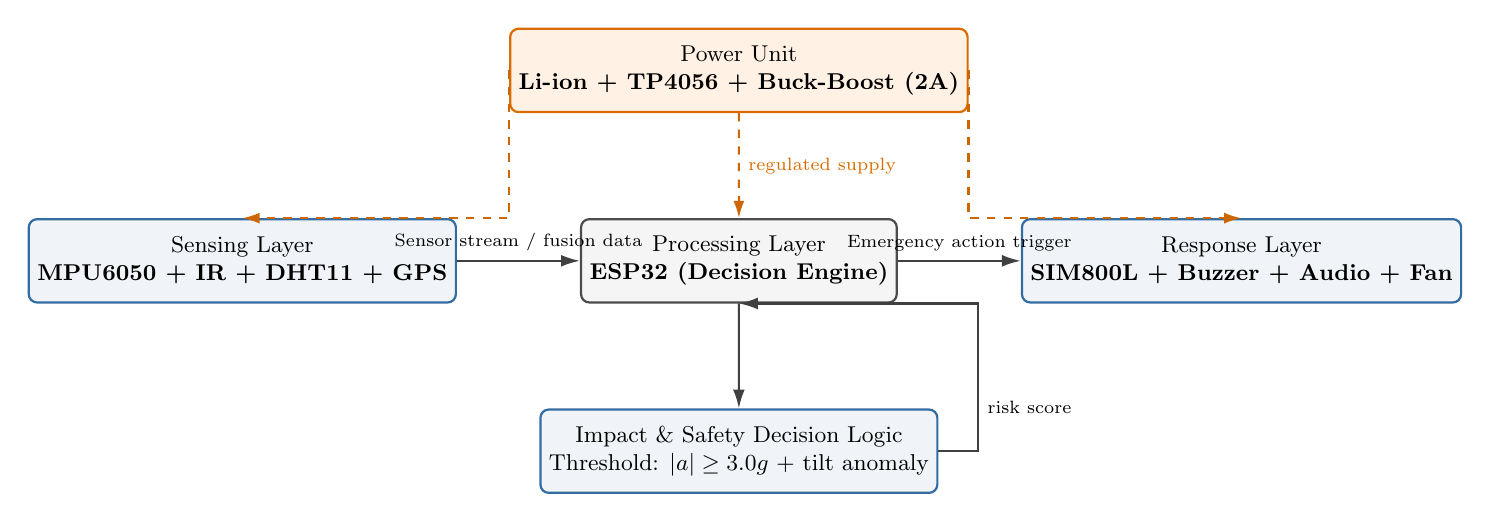
\begin{tikzpicture}[
  scale=0.92, transform shape,
  node distance=1.4cm and 1.7cm,
  module/.style={draw=accentblue!80, rounded corners=3pt, thick, fill=accentblue!6, align=center, minimum width=3.6cm, minimum height=1.15cm, font=\small},
  process/.style={draw=black!70, rounded corners=3pt, thick, fill=gray!8, align=center, minimum width=4.3cm, minimum height=1.15cm, font=\small},
  line/.style={-{Latex[length=2.4mm,width=1.5mm]}, thick, draw=black!75},
  pwr/.style={-{Latex[length=2.2mm,width=1.4mm]}, thick, draw=orange!80!black, dashed}
]

\node[module] (sensor) {Sensing Layer\\\textbf{MPU6050 + IR + DHT11 + GPS}};
\node[process, right=of sensor] (controller) {Processing Layer\\\textbf{ESP32 (Decision Engine)}};
\node[module, right=of controller] (alert) {Response Layer\\\textbf{SIM800L + Buzzer + Audio + Fan}};

\node[module, below=1.45cm of controller, minimum width=4.5cm] (logic) {Impact \& Safety Decision Logic\\Threshold: $|a| \geq 3.0g$ + tilt anomaly};
\node[module, above=1.45cm of controller, minimum width=4.0cm, fill=orange!10, draw=orange!85!black] (power) {Power Unit\\\textbf{Li-ion + TP4056 + Buck-Boost (2A)}};

\draw[line] (sensor) -- node[above, font=\scriptsize] {Sensor stream / fusion data} (controller);
\draw[line] (controller) -- node[above, font=\scriptsize] {Emergency action trigger} (alert);
\draw[line] (controller) -- (logic);
\draw[line] (logic.east) -- ++(0.55,0) |- node[pos=0.15, right, font=\scriptsize] {risk score} (controller.south);
\draw[pwr] (power) -- node[right, font=\scriptsize, text=orange!85!black] {regulated supply} (controller.north);
\draw[pwr] (power.west) |- (sensor.north);
\draw[pwr] (power.east) |- (alert.north);

\end{tikzpicture}
\caption{Professional System Architecture of the IoT-Based Smart Helmet}
\end{figure}

\subsection{Description of Each Module}

\begin{description}[leftmargin=1.5em, labelwidth=0em]

  \item[\textbf{1. Sensing Layer (MPU6050, IR, DHT11, GPS Neo-7M):}]
  The sensing layer provides continuous multi-parameter monitoring. The MPU6050 captures tri-axial acceleration and angular motion for impact/tilt analysis. The IR sensor verifies whether the helmet is worn, preventing false event processing when the helmet is idle. The DHT11 monitors internal helmet temperature for rider comfort management. The Neo-7M GPS module provides latitude-longitude coordinates used for emergency localization.

  \item[\textbf{2. Processing Layer (ESP32):}]
  The ESP32 functions as the main embedded intelligence unit. It performs sensor fusion and event classification by correlating acceleration magnitude, orientation change, and helmet-worn state. A decision threshold (e.g., resultant acceleration $\geq 3.0g$ with abnormal tilt) is used to flag probable crash events. The controller also manages timers, communication sequencing, and fail-safe logic.

  \item[\textbf{3. Communication and Alert Layer (SIM800L + Audio/Buzzer):}]
  On validated emergency detection, SIM800L sends an SMS containing an incident alert and Google Maps location link, followed by an automated call to the configured emergency contact. A buzzer/audio path provides immediate local warning and system-state indication.

  \item[\textbf{4. Thermal Comfort and Safety Actuation:}]
  A 5V DC fan is switched automatically based on helmet temperature (threshold: approximately $30^{\circ}$C). This feature improves rider comfort and demonstrates autonomous environmental response integrated into the safety system.

  \item[\textbf{5. Power Management (TP4056 + Buck-Boost Converter):}]
  The TP4056 manages safe charging of the battery pack, while the buck-boost converter provides stable regulated output for mixed-voltage modules. This ensures reliable field operation despite battery voltage variation.

\end{description}

\subsection{How the Modules Collectively Enable Real-Time Operation}

The modules operate as a closed-loop real-time embedded system. In each control cycle, the ESP32 acquires IMU, IR, temperature, and GPS data; updates accident-risk estimation; checks manual override state; and executes communication/actuation outputs. The sensing-decision loop runs at approximately 50--100 Hz for inertial data, while communication tasks are event-driven. This architecture enables low-latency hazard response while maintaining robust autonomous behavior in practical riding conditions.

% ════════════════════════════════════════════════════════════════════════════
\section{System Design and Implementation}

\subsection{Hardware Components}

\begin{table}[H]
\centering
\renewcommand{\arraystretch}{1.4}
\begin{tabular}{|>{\bfseries}l|l|l|}
  \hline
  \rowcolor{accentblue!12}
  Component & Specification & Role \\
  \hline
  ESP32 Dev Module & Dual-core MCU, WiFi + BLE & Main controller and decision engine \\
  MPU6050 & 3-axis accelerometer + gyroscope & Impact and tilt detection \\
  GPS Neo-7M & GNSS receiver module & Real-time location tracking \\
  SIM800L GSM & Quad-band GSM/GPRS & SMS and call-based emergency alerts \\
  DHT11 & Temperature/Humidity sensor & Helmet microclimate monitoring \\
  IR Sensor & Digital proximity output & Helmet wear detection \\
  TP4056 + Buck-Boost (2A) & Charging + regulated power path & Battery management and voltage stability \\
  Buzzer + BT Audio Amp + Speaker & Audio alert subsystem & Local warning and voice alert interface \\
  5V DC Fan & Brush DC mini fan & Temperature-based cooling \\
  Push Button & Momentary switch & 10-second false-alert cancellation \\
  \hline
\end{tabular}
\caption{Hardware Components Used in the Smart Helmet Prototype}
\end{table}

\subsection{Circuit Connections}

\begin{table}[H]
\centering
\renewcommand{\arraystretch}{1.4}
\begin{tabular}{|l|l|}
  \hline
  \rowcolor{accentblue!12}
  \textbf{Module / Signal} & \textbf{ESP32 Pin} \\
  \hline
  MPU6050 SDA / SCL & GPIO21 / GPIO22 (I\textsuperscript{2}C) \\
  GPS Neo-7M TX / RX & GPIO16 / GPIO17 (UART1) \\
  SIM800L RX / TX & GPIO25 / GPIO26 (UART2) \\
  IR Helmet Detection & GPIO13 \\
  DHT11 Data & GPIO14 \\
  Manual Cancel Button & GPIO12 (INPUT\_PULLUP) \\
  Buzzer Output & GPIO32 \\
  Fan Driver Control & GPIO33 \\
  \hline
\end{tabular}
\caption{ESP32 Pin Mapping for Integrated Modules}
\end{table}

\subsection{Source Code}

\begin{lstlisting}[style=arduino, language=C++, caption={Smart Helmet -- Key Embedded Logic (Abridged)}]
#include <HardwareSerial.h>
#include <Wire.h>
#include <TinyGPS++.h>
#include <DHT.h>

#define BUTTON_PIN 12
#define BUZZER_PIN 32
#define IR_PIN 13
#define MPU_ADDR 0x68
#define DHT_PIN 14
#define FAN_PIN 33

HardwareSerial sim800(2);
HardwareSerial gpsSerial(1);
TinyGPSPlus gps;
DHT dht(DHT_PIN, DHT11);

const char* emergencyNumber = "+919995681865";
bool helmetWorn = false;
bool countdownActive = false;
unsigned long countdownStart = 0;
const unsigned long cancelTime = 10000;
float tempThreshold = 30.0;

void loop() {
  updateGPS();
  checkHelmetStatus();
  checkForIncomingSMS();
  controlHelmetFan();

  if (helmetWorn) detectImpact();

  if (countdownActive && millis() - countdownStart >= cancelTime) {
    sendEmergencyAlert();
    countdownActive = false;
  }
}

void detectImpact() {
  // Read accelerometer (MPU6050)
  float totalAcc = sqrt(ax_g*ax_g + ay_g*ay_g + az_g*az_g);

  if (totalAcc >= 3 && !countdownActive) {
    countdownActive = true;
    countdownStart = millis();
  }
}

void sendEmergencyAlert() {
  String message = "ACCIDENT ALERT!\n";
  message += "Helmet worn and accident detected.\n";
  message += getCurrentLocationLink();
  sendSMS(emergencyNumber, message.c_str());
  makeCall(emergencyNumber);
}

void controlHelmetFan() {
  if (!helmetWorn) { digitalWrite(FAN_PIN, LOW); return; }

  float temperature = dht.readTemperature();
  if (!isnan(temperature) && temperature > tempThreshold)
    digitalWrite(FAN_PIN, HIGH);
  else
    digitalWrite(FAN_PIN, LOW);
}
\end{lstlisting}

\subsection{Working Principle}

The working sequence is event-driven and safety-prioritized. First, the ESP32 continuously reads IMU acceleration/gyro values, helmet-wear status from the IR sensor, and periodic GPS/DHT11 data. Second, a sensor-fusion stage computes resultant acceleration and orientation change to detect crash-like behavior. If impact thresholds are crossed while the helmet is worn, the controller starts a 10-second cancellation timer and activates local warning. Third, if the rider presses the manual button within the window, the alert is aborted as a false positive. Otherwise, the system autonomously sends an emergency SMS containing a Google Maps link and initiates a GSM call to the registered contact. Parallelly, thermal control logic enables the fan when helmet temperature exceeds the configured threshold, maintaining rider comfort during operation.

% ════════════════════════════════════════════════════════════════════════════
\section{Demonstration and Performance Analysis}

\subsection{Prototype Demonstration}

The prototype was integrated into a standard full-face helmet enclosure. The ESP32, SIM800L, and power subsystem were mounted in a protected rear compartment, while the MPU6050 and IR sensor were positioned to accurately capture head motion and helmet-wear state. The Neo-7M GPS antenna was routed to an exposed top section for improved sky visibility, and the fan was mounted near the vent channel for airflow assistance. The final assembly remained lightweight and suitable for real-world riding trials.

\begin{figure}[H]
\centering
\includegraphics[width=0.42\textwidth]{robo_proj.png}
\caption{Smart Helmet Prototype Used for Demonstration}
\end{figure}

\subsection{Test Scenarios Evaluated}

\begin{enumerate}[leftmargin=1.5em]

  \item \textbf{Simulated High-Impact Event:} A controlled shock profile (helmet drop + abrupt deceleration test) produced resultant acceleration above $3.0g$, correctly triggering countdown mode and alert pipeline.

  \item \textbf{False Alert Cancellation:} During non-critical high motion, the manual push-button was pressed within 10 seconds. The system successfully aborted SMS/call transmission.

  \item \textbf{GPS + GSM Emergency Dispatch:} In open-sky outdoor tests, the helmet transmitted SMS alerts with valid Google Maps links and initiated emergency calls in under 12 seconds from event confirmation.

  \item \textbf{Helmet Wear Interlock:} When the helmet was not worn (IR inactive), impact logic remained gated, preventing unintended emergency triggers.

  \item \textbf{Thermal Control Validation:} At internal temperature above approximately $30^{\circ}$C, fan output switched ON automatically and returned OFF once temperature dropped below threshold.
\end{enumerate}

\subsection{Real-Time Performance Analysis}

The inertial monitoring loop executes at approximately 50--100 Hz, which is sufficient for real-time accident dynamics capture. Local event recognition latency was measured in the range of 80--150 ms depending on motion complexity. End-to-end emergency response time (impact confirmation to SMS dispatch) was typically 6--10 s due to intentional fail-safe delay and GSM network overhead. GPS fix reliability improved significantly in open environments, with location accuracy typically within 3--8 m. Overall behavior validates that the prototype meets practical real-time embedded safety requirements.

% ════════════════════════════════════════════════════════════════════════════
\section{Discussion}

\subsection{Enhancement Over Conventional Methods}

Traditional helmets are passive protection devices: they reduce head injury severity but cannot detect crash events, evaluate rider state, or contact emergency responders. The proposed smart helmet adds \textbf{active safety intelligence} through onboard sensing, autonomous event detection, and immediate communication. Compared with conventional helmets, it improves post-accident response time, supports rider survivability in isolated routes, and reduces dependency on bystander intervention.

\subsection{Reduction of Risk to Human Rescuers / Caregivers}

By automatically initiating alerts after severe incidents, the system can reduce response burden on bystanders, traffic personnel, and emergency operators during the critical golden period. The 10-second manual override also protects responders from unnecessary dispatches triggered by non-critical events.

\subsection{Societal Relevance}

The Smart Helmet addresses a major public-health challenge in road safety. It supports safer commuting for students, delivery riders, and long-distance two-wheeler users. The same architecture is adaptable to industrial helmets for mining, construction, and hazardous-site workers where fall/impact detection and instant incident reporting are critical.

\subsection{Alignment with Sustainable Development Goals (SDGs)}

\begin{description}[leftmargin=1.5em]

  \item[\textbf{SDG 3 -- Good Health and Well-Being:}]
  The prototype improves trauma-response readiness by accelerating emergency notification and location sharing after crashes, directly supporting reduced mortality and injury severity.

  \item[\textbf{SDG 9 -- Industry, Innovation and Infrastructure:}]
  The project demonstrates practical embedded innovation by integrating sensing, communication, and autonomous control into a scalable smart safety product for mobility infrastructure.

  \item[\textbf{SDG 11 -- Sustainable Cities and Communities:}]
  Smart rider-safety systems contribute to safer transport ecosystems by enabling faster emergency response and data-driven safety integration in connected urban mobility.

\end{description}

% ════════════════════════════════════════════════════════════════════════════
\section{Limitations and Future Enhancements}

\subsection*{Limitations}
\begin{itemize}[leftmargin=1.5em]
  \item GSM dependency can increase alert latency in weak-network zones.
  \item GPS precision degrades in tunnels, dense urban canyons, or heavy weather conditions.
  \item Rule-based thresholding may still generate occasional false positives/negatives under extreme riding behavior.
  \item Battery backup depends on communication load and must be sized for long rides.
\end{itemize}

\subsection*{Future Enhancements}
\begin{itemize}[leftmargin=1.5em]
  \item \textbf{AI-Based Crash Classification:} Deploy TinyML models on ESP32 to differentiate potholes, hard braking, and true crashes.
  \item \textbf{Mobile Application Integration:} Add BLE/WiFi companion app for live tracking, health telemetry, and configurable emergency contacts.
  \item \textbf{Cloud and Fleet Analytics:} Store anonymized event logs for hotspot analysis and preventive road-safety planning.
  \item \textbf{Smart Vehicle Integration:} Interface with motorcycle ECU/CAN gateway for richer contextual safety decisions.
  \item \textbf{Expanded Use Cases:} Adapt firmware profile for industrial worker helmets and emergency response teams.
\end{itemize}


% ════════════════════════════════════════════════════════════════════════════
\section{Conclusion}

The IoT-Based Smart Helmet for Rider Safety and Emergency Response was successfully designed, implemented, and validated as a real-time embedded safety prototype. By integrating ESP32 control, IMU-based accident sensing, GPS localization, GSM emergency communication, wear-state verification, and thermal actuation, the system demonstrates autonomous end-to-end emergency handling with practical field relevance.

The implemented fail-safe mechanism (10-second manual override) improves operational reliability by reducing false emergency dispatches, while automated location-linked alerts improve rescue readiness. Overall, the project demonstrates a technically sound and deployable engineering solution aligned with modern intelligent transportation safety needs, and it provides a strong foundation for AI-enhanced next-generation smart helmet systems.


% ════════════════════════════════════════════════════════════════════════════
\section*{References}
\addcontentsline{toc}{section}{References}

\begin{enumerate}[leftmargin=1.5em, label={[\arabic*]}]
  \item Espressif Systems, \textit{ESP32 Series Datasheet}, latest revision.
  \item TDK InvenSense, \textit{MPU-6000/MPU-6050 Product Specification}, Rev. 3.4.
  \item SIMCom Wireless Solutions, \textit{SIM800L Hardware Design Guide}, latest revision.
  \item u-blox, \textit{NEO-7 GNSS Modules Data Sheet}, latest revision.
  \item Aosong Electronics, \textit{DHT11 Temperature and Humidity Sensor Datasheet}.
  \item World Health Organization, \textit{Global Status Report on Road Safety}, latest edition.
  \item United Nations, \textit{Sustainable Development Goals}, \url{https://sdgs.un.org/goals}, accessed 2026.
\end{enumerate}

\end{document}
